% !TEX root = ../../my-thesis.tex
\newcommand{\perr}{|\nicefrac{(\hat p -\Tilde{p})}{\Tilde{p}}|}
\newcommand{\by}{\textbf{y}}
\newcommand{\AIC}{\text{AIC}}
\newcommand{\M}{\mathcal{M}}

\graphicspath{{./content/chap3_mini-batching/}}

%
\chapter{Mini-batching ecological data to improve ecosystem models with machine learning}
\label{chap:mini-batching}

by Victor Boussange$^{1,2}$, 
Pau Vilimelis Aceituno$^{3}$, 
and 
Loïc Pellissier$^{1,2}$\bigskip\\

$^1$ \small{Swiss Federal Research Institute WSL, CH-8903 Birmensdorf, Switzerland}\smallskip\\
$^2$ \small{Landscape Ecology, Institute of Terrestrial Ecosystems, Department of Environmental System Science, ETH Zürich, CH-8092 Zürich, Switzerland}\smallskip\\
$^3$ \small{Institute of Neuroinformatics, ETH Zürich and University of Zürich, Zürich, Switzerland}\smallskip

\begin{center}
    \href{https://www.biorxiv.org/content/10.1101/2022.07.25.501365v1}{bioRxiv:2022.07.25.501365}\\
    In review at PLOS Computational Biology
\end{center}

\fancyabstract{
Ecosystems are involved in global biogeochemical cycles that regulate climate and provide essential services to human societies.
%
Mechanistic models are required to describe ecosystem dynamics and anticipate their response to anthropogenic pressure, but their adoption has been limited in practice because of issues with parameter identification and because of model inaccuracies. 
%
While observations could be used to directly estimate parameters and improve models, model nonlinearities as well as shallow, incomplete and noisy datasets complicate this process. 
%
Here, we propose a machine learning (ML) framework relying on a mini-batch method combined with automatic differentiation and state-of-the-art optimizers. By splitting the data into mini-batches with a short time horizon, we show both analytically and numerically that the mini-batch method regularizes the learning problem. When combined with the proposed numerical implementation, the resulting ML framework can efficiently learn the parameters of complex dynamical models and is a workhorse for model selection. 
%
We evaluate the performance of the ML framework in recovering the dynamics of a simulated food-web. We show that it can efficiently learn from noisy, incomplete and independent time series, accurately estimating the model parameters and providing reliable short-term forecasts. We further show that the ML framework can provide statistical support for the true generating model among several candidates. 
%
In summary, the proposed ML framework can efficiently learn from data and elucidate mechanistic pathways to improve our understanding and predictions of ecosystem dynamics.}


\section{Introduction}

%%
Ecosystems are complex systems involving many interacting functional entities which together play a major role in regulating global biogeochemical cycles \citep{Bonan2008} and delivering essential services to humans \citep{Kremen2005}.
%
Ecosystems currently face intense disruption from anthropogenic pressure, through pollution and land use \citep{Doney2010,Ellis2011}, and from climate change \citep{Midgley2019}. In order to anticipate the responses of ecosystems to these disruptions, models that can extrapolate ecological dynamics beyond observations are required \citep{Boyd2012}. 
%
A major challenge is that the processes driving ecological dynamics are nonlinear, resulting in complex responses and feedbacks \citep{Scheffer2001}. Nonlinearity greatly affects the capacity of modelling approaches that do not incorporate specific biological knowledge to reliably project current trends into the future \citep{Barnosky2012}. For instance, while methods based on statistical descriptions \citep{Deneu2021} and nonparametric methods \citep{Ye2015,Ye2016,Deyle2016} have adequate interpolation capabilites, they are ill-suited for extrapolating beyond observed trends \citep{Barnosky2012,Urban2016}.
%
In contrast, mechanistic ecosystem models integrate constraints on the expected dynamics by explicitly modelling interactions, feedback loops and dependencies between ecosystem components \citep{Geary2020}. While this should ensure a more robust forecast under large disruptions \citep{Norberg2012}, ecosystems models suffer in practice from parametrization issues, i.e. inaccuracies in the mathematical formulation of the processes and issues in identifying the correct parameter values \citep{DeAngelis2015}. These drawbacks have limited their broad adoption \citep{Urban2016}.
%
Learning the parametrization of ecosystem models from observation data by blending specific biological knowledge and ML methods could improve our representation of ecosystem processes and help us to anticipate ecosystem responses to global changes.

%%
% 2nd paragraph
The parametrization of ecosystem models can be indirectly learnt from observations by calibrating the parameters from the data collectively using inference methods. These methods proceed by maximizing the posterior probability of the parameters given the observations, but their success is subject to a number of issues, some of which specifically relating to ecosystem model properties.
%
Among these issues, the exploration of the posterior landscape demands repeated model simulations, but ecosystem models are usually associated with a high computational cost that limits the number of possible runs \citep{Fisher2018}. 
%
Additionally, the complexity of processes requires a large number of parameters. Due to the curse of dimensionality \citep{Boyd2012}, this complicates the exploration of the posterior distribution and can further leave many parameters poorly constrained \citep{Gutenkunst2007}. The limited availability of observations, which are usually composed of multiple partial short-term time series \citep{Scheiter2013,Schartau2017}, accentuates the lack of parameter constraints. 
%
Moreover, ecosystem dynamics can be strongly dependent on the initial conditions (ICs) and show a chaotic behaviour \citep{Hastings1993,Huisman1999,Beninca2008}, or can be associated with a large panel of dynamics depending on the parameter values. In such case, small perturbations of the ICs or parameter values lead to large divergences in the model outcomes, causing numerical problems in finding the most probable parameters \citep{DeAngelis2015}.
%
Last but not least, in contrast to fields such as climate and weather modelling, the derivation of fundamental processes regulating ecosystems is far from being established \citep{Gehlen2015,Schartau2017,Purves2013}, resulting in inaccurate mechanistic pathways and uncertain mathematical formulations \citep{Gentleman2003}, limiting extrapolation to unseen data.
%
To summarize, the parametrization of ecosystem models requires inference methods that are robust despite the models' complexity, the limited observation data, and the inaccurate description of ecological processes.

%%
% 3d paragraph
A variety of data assimilation and ML methods are increasingly being used to parametrize ecosystem models.
%
Bayesian inference with Markov Chain Monte Carlo methods, used in \citep{Lignell2013,Higgins2010,Xu2006,Fiechter2013,Rosenbaum2019}, offer the advantage of quantifying uncertainties by inferring the full posterior probability distribution of the unknown parameters. This is achieved by a global exploration of the parameter space, which makes Bayesian methods computationally expensive and particularly prone to the curse of dimensionality \citep{Gosh2021}.
%
Simulated annealing \citep{Matear1995}, genetic algorithms \citep{Ward2010}, and sequential methods such as extended Kalman filtering and ensemble Kalman methods \citep{Bertino2003,Doron2013,Gharamti2017} have been used as alternatives, but are similarly subject to the curse of dimensionality and demand a large number of model evaluations.
%
Variational methods rely on the model adjoint, i.e. the model sensitivity to the parameters, to explore more efficiently the parameter space, iteratively updating the parameter estimates using the gradient of the posterior landscape. Such methods therefore demand less evaluation \citep{Schartau2017}, which explains their wide adoption in the field of artificial intelligence to train highly parametrized neural networks (up to the order of $10^8$ parameters \citep{NIPS2017_3f5ee243}) and their use in calibrating marine ecosystem models \citep{Fennel2001,Spitz1998,Xiao2014,Pelc2012} (see \citep{Schartau2017} for a review) and terrestrial ecosystem models \citep{Zhu2015,DeLong2014,Curtsdotter2019}. 
%
However, as the complex dynamics of ecosystem models tend to be associated with rugged posterior landscapes, variational methods are prone to converging to local minima, making variational methods very sensitive to the choice of initial model parameters \citep{Gabor2015,Schartau2017}.
%
Ecosystem models are specified as differential equations that depend not only on parameters but also on ICs. The state-dependency of ecosystems means that neglecting the estimation of initial ICs might compromise the correct fitting of the parameters and the forecast skill \citep{Lignell2013}. However, few of the aforementioned studies have addressed the problem of IC estimation (but see \citep{Pelc2012}). 
%
Finally, the numerical implementation of variational methods is also challenging, as the model adjoint is difficult to obtain and maintain as the model is modified \citep{Lawson1995,Pelc2012,Gharamti2017}. 
%
Novel methods for model parametrization are emerging, thanks to advances in the field of artificial intelligence \citep{Willard2020,Kashinath2021,Alber2019,Peng2021}, providing new opportunities to better address these issues.
    
%%
% 4th paragraph    
Here, we propose a ML framework relying on a mini-batch method inspired by multiple shooting methods \citep{Pisarenko2004} and on automatic differentiation and state-of-the-art optimizers to efficiently learn the parametrization of ecosystem models from observation data. 
%
The mini-batch method divides the training problem into mini-batches with a short time horizon. We show analytically how this learning strategy regularizes the ill-behaviour of the loss function arising from the strong nonlinearities of ecosystem models.
%
We implement the mini-batch method in the software ecosystem SciML \citep{Rackauckas2020a}, which provides advanced optimizers and allows the automatic generation of efficient and accurate model adjoints, leading to excellent performance.
%
The resulting ML framework makes it possible to efficiently combine the information contained in short, independent time series, and is a workhorse for performing model selection and improving model accuracy.
%
We evaluate the performance of the ML framework in recovering the chaotic dynamics of simulated food webs. We assume a perfect-model setting and test the capacity of the ML framework to recover the true parameters and provide forecasts based on noisy and incomplete observations, and we explore its efficiency in combining the information from multiple time series. Additionally, we investigate whether the ML framework can recover the most appropriate model structure among candidate models. 
%
By blending biological knowledge and ML methods, the proposed ML framework is interpretable and data-efficient, and it facilitates mechanism discovery. The proposed approach thus shows promise in improving our ability to understand and forecast ecosystem dynamics.

\section{Machine learning framework for ecosystem models}\label{sec:methods}
\subsection{Ecosystem model parametrization as a learning problem}
\subsubsection{Ecosystem models}
Ecosystem models generally consist of a system of ordinary differential equations (ODEs) of the form
\begin{equation}\label{eq:prob_statement}
    \begin{split}
        &\dot{x}(t) = f(t, x(t), p)\\
        &x(0) = x_0\\
        &y(t) = h(x(t)) + \epsilon(t)\\
    \end{split}
\end{equation}
%
where $x(t) \in \R^m $ is a vector of state variables that might represent species abundance, resources availability or functional group biomass, $y(t) \in \R^d$ is a vector of observables that contains a subset or aggregates of the state variables, and $p \in \R^q$ is the model parameter vector.
% 
$h$ is a function that maps the state variables to the observables, and we assume that the observables are contaminated with a white noise $\epsilon$ of Gaussian type, with zero mean and variance--covariance matrix $\Sigma_y$. 
%
Denoting by $\theta = (x_0, p)$ the vector containing the ICs and the parameters, the model may be viewed as a map $\M$ parametrized by time $t$ that takes the parameters $\theta$ to the state variables $x$
\begin{equation}
\begin{split}
        \M(t,\theta) &= x(t) \\
            &= \int_0^t f(s, x(s), p) ds + x_0
\end{split}
\end{equation}

\subsubsection{Inverse modelling}
Taking expectations over the noise realizations yields $ \E [y(t)] = h(\M(t,\theta))$, and it follows that the conditional likelihood of each observation $y_k \equiv y(t_k)$, given the parameters $\theta$ and the model $\M$ denoted by $p( y_k | \theta, \M )$, follows the distribution of the residuals $\epsilon_k \equiv \epsilon(t_k) = y(t_k) - h\left(\M(t_k, \theta)\right)$, which corresponds to the multivariate normal distribution $\mathcal{N}_{0, \Sigma_y}$.
%
Following a Bayesian approach, the parametrization of the ecosystem model can be performed on the basis of the parameter and model posterior probability $p(\theta, \M | \by_{1:K})$, i.e. the conditional probability density of the parameter values $\theta$ and the model $\M$ given the data, given by 
\begin{equation}
    p(\theta, \M | \by_{1:K}) \propto p(\by_{1:K} | \theta, \M) p(\theta, \M)
\end{equation}
where $\by_{1:K} = (y_1,\dots,y_K)$, $p(\by_{1:K} | \theta, \M)$ is the product of the conditional likelihood of each observation $y_k$
\begin{equation}
\begin{split}
    p(\by_{1:K} | \theta, \M) &= \prod_{i=1}^K p(y_{i} | \theta, \M)\\
                        &= \prod_{k=1}^K \frac{1}{\sqrt{(2\pi)^d|\Sigma_y|}} \exp \left(-\frac{1}{2} \epsilon_k^{T} \Sigma_y^{-1} \epsilon_k \right)
\end{split}
\end{equation}
and $p(\theta,\M)$ is the prior distribution of the model and its associated parameter values. The model $\M$ is included in the probabilistic quantities in order to accommodate multiple candidate models (see \cref{sec:model_comparision}).

A variational method to obtain a Bayesian estimate of $\theta$ involves maximizing $p(\theta, \M | \by_{1:k})$ to obtain the maximum a posteriori (MAP) estimator \citep{Bocquet2019}, which is equivalent to a maximum likelihood approach under a uniform prior distribution of the parameters, i.e. when no prior information on the parameter values is used \citep{Schartau2017}. Observing that maximizing $p(\theta, \M | \by_{1:K})$ is equivalent to minimizing $- \log p(\theta | \by_{1:K}, \M)$ and assuming a normal prior distribution of the parameters $\mathcal{N}_{p_b, \Sigma_p}$, one can obtain the MAP $\hat{\theta}$
\begin{equation}\label{eq:argmin_xi}
    \hat{\theta} = \argmin_\theta  L_{\M}(\theta)
\end{equation}
%
where 
\begin{equation}\label{eq:loss_fn}
    \begin{split}
    L_{\M}(\theta) &= \frac{1}{2} \left[ \sum_{k=1}^{K-1} \|y_k - h\left(\M(t_k,\theta)\right)\|_{\Sigma_y}^2 + \|p - p_b\|_{\Sigma_p}^2 \right] \\
   \end{split}
\end{equation}
\citep{Schneider2017,Raue2009} and where we use the notation $\|y\|_\Sigma^2 = y \Sigma^{-1}y^{\textbf{T}}$.
%
\cref{eq:loss_fn} is similar to a traditional least squares function commonly used in regression, where the second summand is the analogue of a regularization term for the weights and biases of e.g. a neural network.

%
Gradient-based optimizers can then be used to efficiently obtain $\hat{\theta}$ in \cref{eq:argmin_xi}, iteratively updating the parameter vector $\theta_m$ given the gradient of the loss function, denoted by $\nabla_\theta L_{\M}$, to navigate the surface defined by $L_\M$ with the aim to find the global minimum where $\nabla_\theta L_{\M}(\hat{\theta}) = 0$. 
% 
As an example, the plain vanilla gradient descent algorithm is given by
\begin{equation}\label{eq:SDG}
    \theta_{m+1} = \theta_{m} - \gamma \nabla_\theta L_\M({\theta_m})
\end{equation}
where $\gamma$ is the learning rate. Other gradient-based algorithms, such as the ADAM optimizer used in the section below, employ more advanced updating strategies to avoid convergence to local minima but stay in the spirit of \cref{eq:SDG}.

\subsubsection{Information indigestion}
A naive minimization of $L_\M(\theta)$ with gradient-based methods is likely to fail, as its associated surface cannot be navigated properly. As illustrated in \cref{fig:training_on_mini-batches}\textbf{A}, the loss surface associated with models characterized by complex dynamics consists of multiple local minima, which cause problems of convergence in efforts to reach the global minimum (depicted by the orange curve in \cref{fig:training_on_mini-batches}\textbf{B}). Furthermore, in a neighbourhood of the global minimum, the gradient of the loss function is very large (a "ravine" with almost vertical walls), leading the optimizer to overshoot the true parameter values (depicted by the green curve in \cref{fig:training_on_mini-batches}\textbf{B}).
%
In \cref{secSI:supmat} we show in a general setting that these problematic features arise from the dynamical properties of ecosystem models: when the dynamics are chaotic or exhibit a limit cycle (as is often the case for ecological dynamics \citep{Bjornstad2001,Hastings1993,Huisman1999,Beninca2008}), the dynamical trajectories exhibit high sensitivity to the model parameters and ICs. This means that a small modification of the parameters or ICs leads to large divergences over time. 
%
The prevalence of large deviations causes discontinuities, appearing as many sub-optimal local minima on the loss surface. Moreover, the true minimum can only be found in a narrow ravine that becomes narrower as the number of data points increases.
% 
Such surfaces are hardly navigable with gradient descent methods, but since the behaviour of $L_\M(\theta)$ critically depends on the time horizon, we reformulate \cref{eq:loss_fn} in the following section by splitting the time series into mini-batches with a short time horizon. 

\subsection{ML framework for ecosystem models}

\subsubsection{Description of the mini-batch method}
We propose a mini-batch method that splits the data into mini-batches with a short time horizon. Under perturbed parameters and ICs, chaotic or limit cycle dynamics only diverge after some characteristic simulation time; by splitting the time series into small mini-batches, discontinuities that cause the poor navigability of the landscape are therefore avoided. By averaging the associated losses during the training, the mini-batch method regularizes the loss function and makes it possible to combine the information contained in independent time series.

Consider the availability of $S$ independent time series, where each time series $s \in \{1,\dots,S\}$ contains $K^{(s)}$ observations $\by_{1:K^{(s)}}^{(s)}$. To improve the ill-behaviour of \cref{eq:loss_fn}, we split each time series into $M^{(s)}$ mini-batches, each of which defines a loss denoted by $L_\M^{(s,m)}$.
%
Averaging the losses $L_\M^{(s,m)}$ leads to a reformulation of the loss function in \cref{eq:loss_fn}, yielding
%
\begin{equation}\label{eq:ML-framework}
    \begin{split}
        L_\M^\star(\theta) &=  \textstyle \frac{1}{S}\sum_{s=1}^{S} \frac{1}{M^{(s)}} \textstyle \sum_{m=0}^{M^{(s)}-1} L_\M^{(s,m)}(\theta)\\
        &= \textstyle \frac{1}{S} \textstyle \sum_{s=1}^{S} \frac{1}{M^{(s)}} \textstyle \sum_{m=0}^{M^{(s)}-1} \Big[ \textstyle \frac{1}{K^{(s,m)}}  \sum_{k=1}^{K^{(s,m)}} \|y_{k + m K^{(s)} / M^{(s)}}^{(s)} - h\left(\M(t_{k + m K^{(s)}}, p, x_{0}^{(s,m)})\right)\|_{\Sigma_y} \\
        & \qquad 
        + \|y_{m K^{(s)} / M^{(s)}}^{(s)} - h\left(x_{0}^{(s,m)}\right)\|_{\Sigma_{x_0}} 
        + \|p_b -  p\|_{\Sigma_p} \Big]
    \end{split}
\end{equation}
%
where 
% 
$\theta = (p, x_{0}^{(1,1)}, \dots  x_0^{(1,M_1)}, x_{0}^{(2,1)} \dots, x_{0}^{(S,M_S)})$ 
%
consists of the augmented parameter vector containing 
%
$\sum_{s=1}^S \left[ M^{(s)} -1 \right]$ 
%
additional ICs to be estimated and denoted by  $x_{0}^{(s,m)}$, 
% 
$K^{(s,m)} = \begin{cases} K^{(s)} / M^{(s)} + 1 &\quad \colon m < M \\ 
                    K^{(s)} / M^{(s)} &\quad \colon m = M
        \end{cases}$ 
% 
% 
indicates the number of points to include in the $m$th batch, and 
% 
$p_b$ 
% 
designates the prior knowledge of the parameter values. 
% 
We refer to \cref{fig:training_on_mini-batches}\textbf{C} for a graphical representation of \cref{eq:ML-framework}.
%
In contrast to \cref{eq:loss_fn}, the ICs for each batch are constrained by an extra term with weight $\Sigma_{x_0}^{-1}$, which is needed in practice for better convergence.
% 
The ICs $x_{0}^{(s,m)}$ are nuisance parameters that augment the dimensionality of the parameter space as they are inferred for each batch. Nonetheless, the efficiency of gradient-based methods, together with the suggested numerical implementation detailed in the section below, largely circumvent the additional cost associated with the augmented dimensionality.
% 
$K^{(s,m)}$ expresses the overlap between each batch of data for $m < M^{(s)}$ and ensures that all the available information is utilized to constrain the parameter vector $p$.
%
By smoothing the ruggedness of the loss surface (orange curve in \cref{fig:training_on_mini-batches}\textbf{A}), the proposed mini-batch method yields an improved navigability (orange curve in \cref{fig:training_on_mini-batches}\textbf{B}). We show analytically in \cref{secSI:supmat} that using $L_\M^\star$ yields a more navigable loss surface than if $L_\M(\theta)$ is used in \cref{eq:loss_fn}.

\begin{figure}[h]
    \centering
    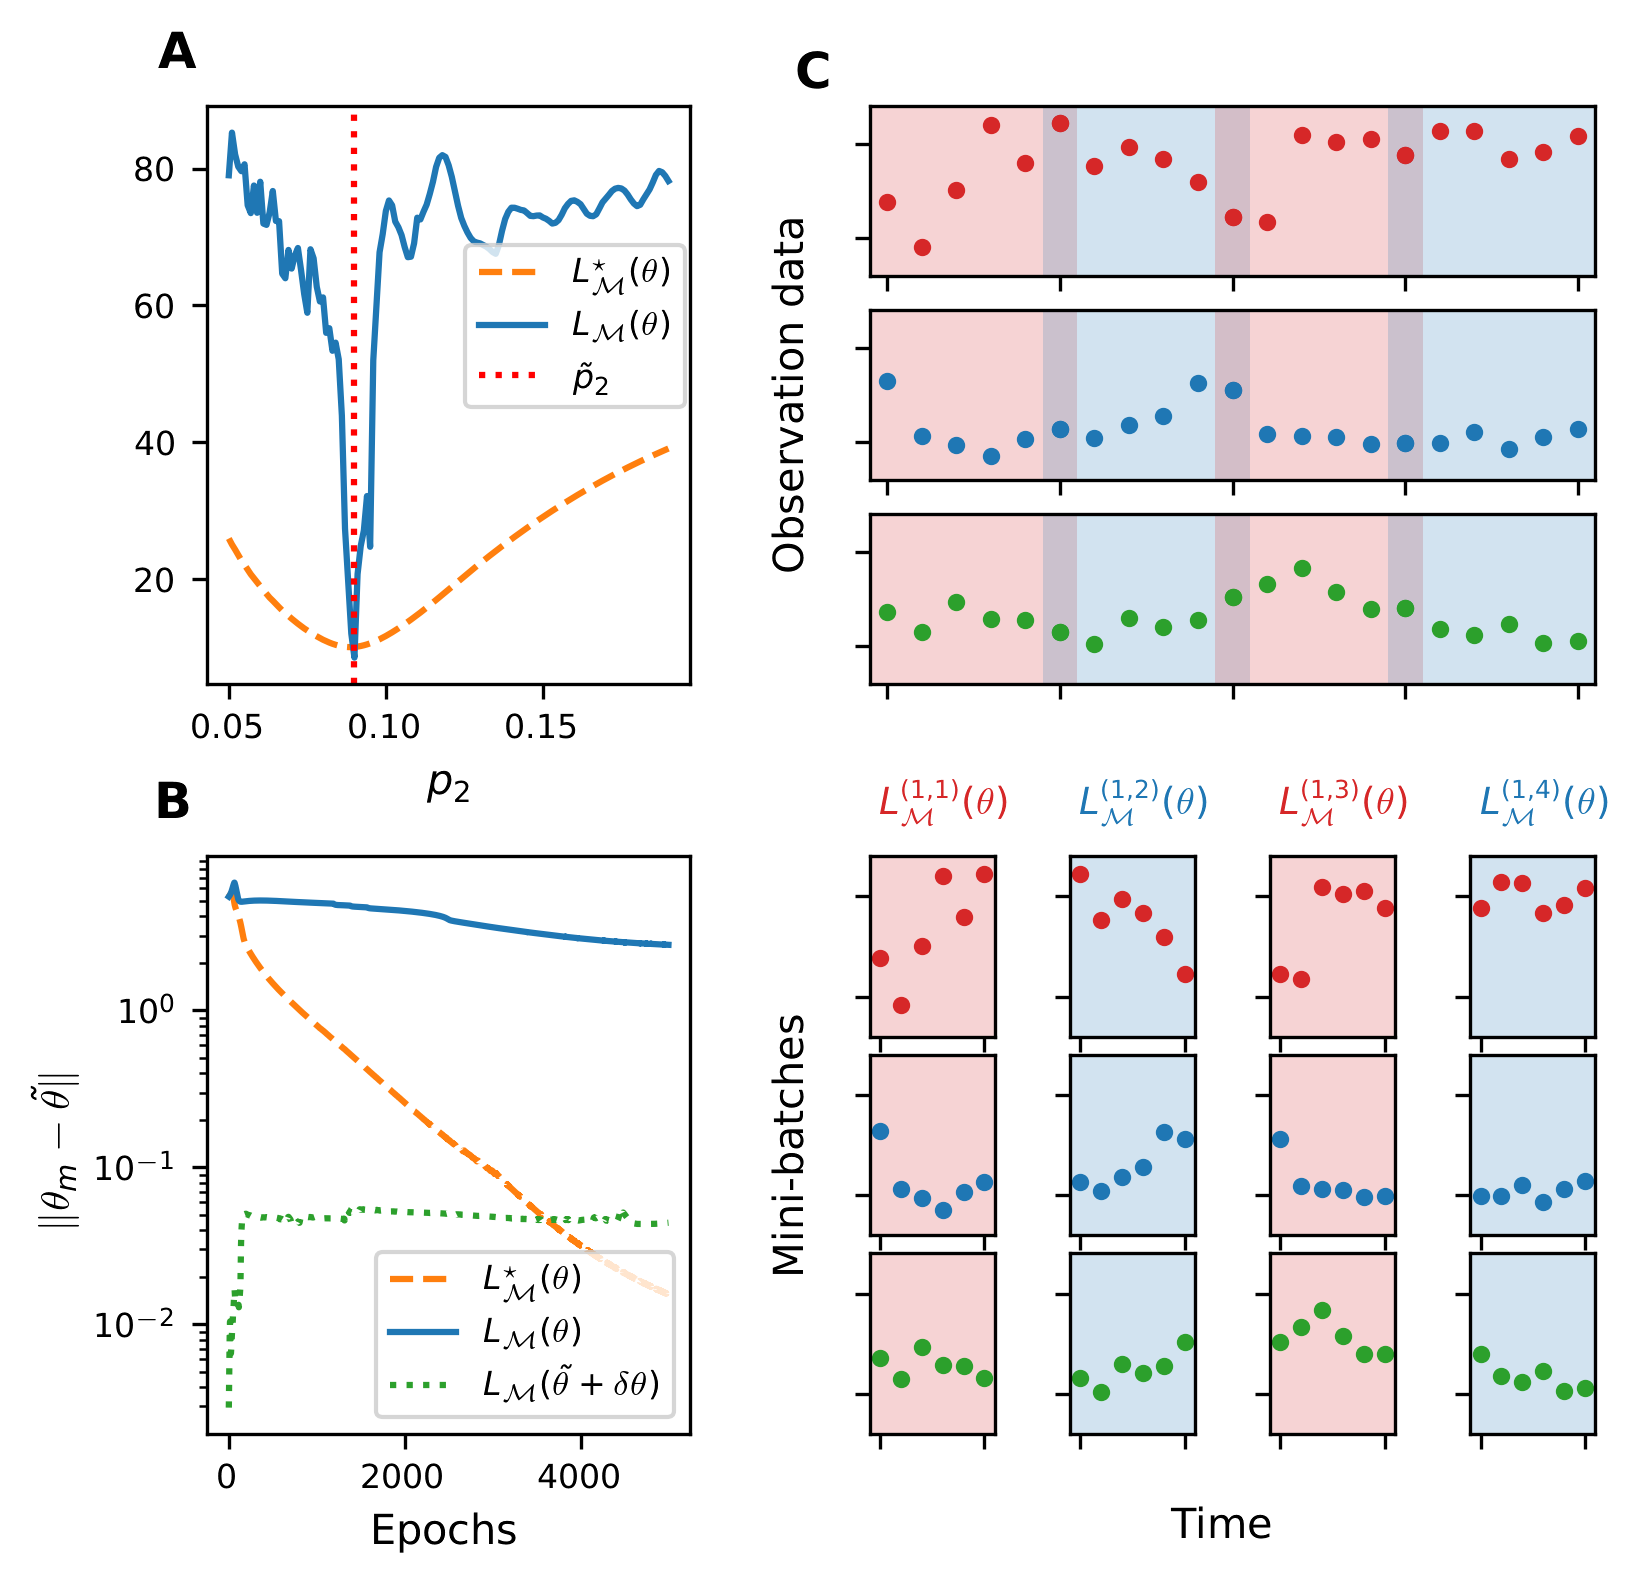
\includegraphics[]{figures/figure1.png}
    \caption{\textbf{Illustration of the mini-batch method.} 
    %
    \textbf{A} Characteristic features of the naive loss function $L_{\M}(\theta)$ and the mini-batch loss function $L_{\M}^\star(\theta)$. The blue and orange lines correspond to cross sections of $L_\M(\theta)$ and $L_\M^\star(\theta)$, respectively, obtained from the ecosystem model presented in the section \nameref{sec:numerical_simulations}. While the cross section of $L_\M(\theta)$ presents many local minima and a very large gradient in the neighbourhood of the true parameter, which renders the navigability of the loss surface difficult, the cross section of $L_\M^\star(\theta)$ is smooth and shows a single minimum, illustrating the regularization induced by the mini-batch method. 
%
    %
    \textbf{B} Convergence of gradient descent algorithms applied to $L_{\M}$ and $L_{\M}^\star$. The blue, orange and green lines correspond to the loss function evaluated against the epochs (number of parameter updates) using $L_{\M}$, $L_{\M}$ starting from a parameter value close to the true parameters, and $L_{\M}^\star$, respectively. The ill-behaviour of $L_\M$ leads to the convergence to a local minimum, while  $L_{\M}^\star$ is associated with a smooth convergence to the true parameters.
    %
    \textbf{C} Graphical representation of the proposed mini-batch method. To improve the navigability of the posterior landscape, the algorithm splits the time series into mini-batches with short time horizons (blue and red portions of the time series). Since mini-batches are treated independently, the method naturally extends to independent time series.}
    \label{fig:training_on_mini-batches}
\end{figure}
\FloatBarrier

\subsubsection{Numerical implementation of the ML framework}

The choice of the optimizer and the correct calculation of the model sensitivity to the parameters and ICs, upon which the gradient of the loss function $\nabla L^\star_\M(\theta)$ depends, play an essential role in the success of the minimization of the loss function and the subsequent correct estimation of the MAP. 
% 
To accelerate the learning process and make it more robust, we propose to combine the mini-batch method with modern optimizers and automatic differentiation.
%
Building upon the software ecosystem SciML \citep{Rackauckas2020a}, we use \textbf{DifferentialEquations.jl} for the forward integration of the ecosystem model, as it provides highly efficient ODE solvers \citep{Rackauckas2017}.  \textbf{DifferentialEquations.jl} is additionally compatible with automatic differentiation and includes an extensive set of sensitivity analysis methods \citep{Ma2021}, enabling the automatic generation of the model sensitivity to the parameters and ICs and guaranteeing their accuracy. This automatic generation greatly reduces the effort and potential errors associated with the adjoint code construction, enabling continuous development of the models. The accuracy is also an essential feature, as the model sensitivities are critically involved in the minimization of \cref{eq:loss_fn} and their inaccuracies can compromise the convergence of the gradient-based optimizers \citep{Gholaminejad2019}.
%
The interoperability of the SciML ecosystem further makes it possible to benefit from the tooling of the deep learning library \textbf{Flux.jl} and the nonlinear optimization library \textbf{Optim.jl} \citep{KMogensen2018}, providing state-of-the-art optimizers that are computationally efficient and well suited for highly parameterized models \citep{Ruder2016}.
% 
We use the adaptive, momentum-based Adam optimizer \citep{Kingma2014} to converge in the basin of attraction of the true parameters, which we substitute with the limited memory Broyden–Fletcher–Goldfarb–Shanno optimizer (L-BFGS) \citep{Liu1989} for the final training epochs to ensure faster and more accurate convergence.

%% 
The reformulation of the learning problem in \cref{eq:ML-framework}, together with the numerical implementation suggested above, define the proposed ML framework, which we benchmark with a concrete case scenario in the next section.

\section{Simulated food-web model as a case study}\label{sec:numerical_simulations}

We evaluate the performance of the ML framework by considering a food-web ecosystem composed of three functional compartments including a resource, consumers and predators. 
%
We use a reference model to generate the observation data and first assume a perfect-model setting, evaluating the performance of the ML framework in parametrizing the reference model for different noise levels, with incomplete observations, and with an increasing number of independent time series.
%
Second, we relax the perfect-model assumption by considering two plausible candidate models capturing contrasting hypotheses regarding the ecological processes, and test whether the ML framework can provide support for the true generating model by combining it with information-based model selection.

\subsection{Three-compartment food-web ecosystem}
We use a reference food-web model investigated in \citep{Hastings1991,McCann1994a,McCann1994,Klebanoff1994} where a resource $R$ is eaten by consumers $C$, which in turn are fed upon by predators $P$ (model $\M_1$ in \cref{fig:3species_foodchain_simple}). We further consider an "omnivory variant" of the reference model introduced in \citep{McCann1997}, where predators are omnivorous and can feed upon the resource with a determined strength $\omega$ (model $\M_2$ in \cref{fig:3species_foodchain_simple}). 
%
These models generate fluctuations that resemble the behaviour of observed ecological time series \citep{Bjornstad2001}, they produce chaotic dynamics that are notoriously challenging to forecast for a wide range of realistic parameters \citep{Post2000}, and they have been used as benchmarks for proposed ecosystem forecasting methods (see \citep{Perretti2013,Deyle2016,Ye2016}). 
 
After nondimensionalization, the three-compartment model and the omnivory variant comprise a total of six and nine parameters, respectively: the mass-specific metabolic rate of consumers and predators $x_C$ and $x_P$, the ingestion rate per unit metabolic rate of consumers and predators $y_C$ and $y_P$ (decomposed into $y_{PC}, y_{PR}$ for the omnivory variant), the half saturation densities for the type II functional responses of the consumers and predators $R_0$ (decomposed into $R_0$, $R_{02}$ for the omnivory variant) and $C_0$, and the omnivory strength $\omega$ for the omnivory variant (see \cref{secSI:models} for the ODE details). 
%
Time is nondimensionalized by the resource growth rate and set to the biologically realistic value of 100\% biomass increase per day, so that one unit of time corresponds to one day. The parameters in the simulations are set to the biologically realistic values proposed by \citep{McCann1994,McCann1997}, which additionally ensure that the dynamics of the system are chaotic or show oscillations (see \cref{secSI:models} for details).

We generate the observation data by sampling the simulated ecosystem dynamics and by contaminating the samples with noise. The noise variance--covariance matrix $\Sigma_y$ is set to be diagonal, with entries that are proportional to the sample variances of the observables
\begin{equation}
    \operatorname{diag} \Sigma_y = r^2 [\Var(\Tilde{y}_1), \dots, \Var(\Tilde{y}_d)]
\end{equation}
where $r$ indicates the noise level and $\Tilde{y}$ corresponds to the noiseless data generated with the true parameter values $\Tilde{\theta}$. 
%
We sample the simulated dynamics after a long burn-in time ($t > 500$) to ensure that transient dynamics are not observed.
%
A visual representation of the generated data is displayed in \cref{fig:3species_foodchain_simple}\textbf{B}.
%
We assume a uniform distribution of the parameter priors, and randomly draw initial parameter estimates from a uniform distribution so that the initial parameter estimates follow $\mathcal{U}(0, 2 \Tilde p)$.

%%
We consider two different settings: one where all compartment abundances are observable, i.e. the observing system map $h$ is the identity, and one where only predator and consumer abundances are available, i.e. discarding the resource abundance data.
%
For both settings, structural identifiability is tested with the Julia library \textbf{StructuralIdentifibility.jl} \citep{Dong2021} and verified globally. This means that in theory, the unique observation of predator and consumer abundances carries the information required for a complete characterization of all the model parameters.

%%
For the meta-parameters of the ML framework, we set 
% 
$\Sigma_{x_0} = \frac{M^{(1)}}{K^{(1)}} \Sigma_y$, 
% 
we use Adam with 
% 
$\gamma_m = \one_{[0,2000]}(m) 10^{-1} +\one_{[0,2000]}(m) 10^{-2} + \one_{[0,2000]}(m) 10^{-3} $, $\beta_1 = 0.9$ 
% 
and $\beta_2 = 0.999$ for the first 6000 epochs, where $\gamma_m$ corresponds to the learning rate of the $m$th epoch, and we use L-BFGS for the last 200 epochs.

\begin{figure}[h]
    \centering
    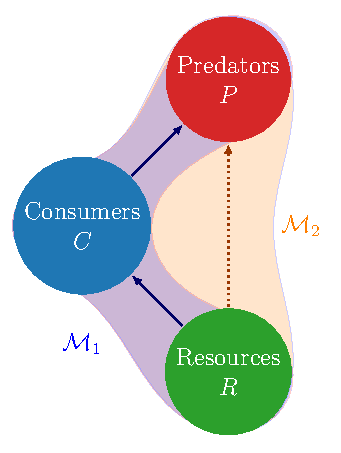
\includegraphics[width=0.3\textwidth]{figures/figure2.pdf}
    \caption{\textbf{Reference food web systems considered.} In \cref{sec:perfect-model}, the blue model $\M_1$ from \citep{Hastings1991} is considered, where a resource is eaten by consumers, which are themselves eaten by predators. In \cref{sec:model_comparision}, the orange model $\M_2$, corresponding to the omnivory variant introduced in \citep{McCann1997}, is also considered.}
    \label{fig:3species_foodchain_simple}
\end{figure}
\FloatBarrier

\subsection{Parameter learning in a perfect-model setting}\label{sec:perfect-model}

We generate time series from the reference food-web model (blue model in \cref{fig:3species_foodchain_simple}) under varying noise levels and for both settings with total and partial observations, sampling from the model simulations every four days (see \cref{fig:training_on_mini-batches}\textbf{C} for an illustration of the generated data).
%
We then apply the ML method to the generated data, with a focus on evaluating its performance in recovering the true parameters $\Tilde{p}$ and on its forecast skill.

%%
We evaluate the performance in recovering the true parameters with two metrics, namely the coefficient of determination between the true parameters $\Tilde x_P$ and the estimated parameters $\hat x_P$, denoted by $R^2_{x_P}$, and the relative parameter error for the ensemble of training simulations, denoted by $\perr$ and calculated as the median relative parameter error across the six estimated parameters.
%
To evaluate the out-of-sample forecast skill, we simulate the model beyond the training time span by using the estimated ICs of the last batch of each independent time series. Further, we quantify the forecast skill, denoted by $\rho^2$, by computing the mean squared correlation across all the independent time series between the prey abundance generated with the true parameter $\Tilde{\theta}$ and the predicted prey abundance.
% 
We obtain summary statistics of the metrics by varying the critical parameter value $x_P$, generating a total of 50 simulations for each noise level and setting considered.  While only $x_P$ is varied, all the parameters together with the ICs are collectively fitted. 

\subsubsection{Robustness of the ML framework against noise and incomplete observations}
We set the number of time series to $S=1$, the time series length to $K = 80$, and the number of mini-batches to $M = 8$. We investigate the ML framework performance against observational noise and under the setting with complete or partial observations.

In the complete observation setting, the ML framework can very accurately recover the true parameter values under a moderate observational noise, with mean $\perr = 6 \%$ and $R^2_{x_P} = 0.99$ for 20\% observational noise ($r = 0.2$; see \cref{fig:perfect_setting_noise}\textbf{A}, red dots).
%
In the partial observation setting, fair results are also obtained with $\perr = 16 \%$ and $R^2_{x_P} = 0.89$ (\cref{fig:perfect_setting_noise}\textbf{A}, blue triangles). 
% 
On top of being accurate, the ML framework further shows a very short inference time, i.e. 36 seconds in the complete observation setting and 34 seconds in the partial observation setting (see \cref{tableSI:simul_time} for details).
% 
To investigate systematically how the ML framework accommodates different levels of observational noise, we vary the noise level from $r = 0.$ to $r = 1$ and calculate $\perr$. Results reported in \cref{fig:perfect_setting_noise}\textbf{B} show that the ML framework handles observational noise well and the response of the logarithm of $\perr$ to $r$ only differs by a constant factor between the complete and partial observation settings.

Given that the food-web dynamics are chaotic (\cref{secSI:models}), excellent performance in parameter estimation might not be sufficient to provide accurate forecasts. We therefore also test the ML algorithm by evaluating how the forecast skill $\rho^2$ is affected by the noise level under complete or partial observations. Results for the complete and partial observation settings reported in \cref{fig:perfect_setting_noise}\textbf{C} show good forecast skill under moderate observational noise, where $\rho^2$ linearly decreases with the time horizon considered. 

\begin{figure}[h]
    \centering
    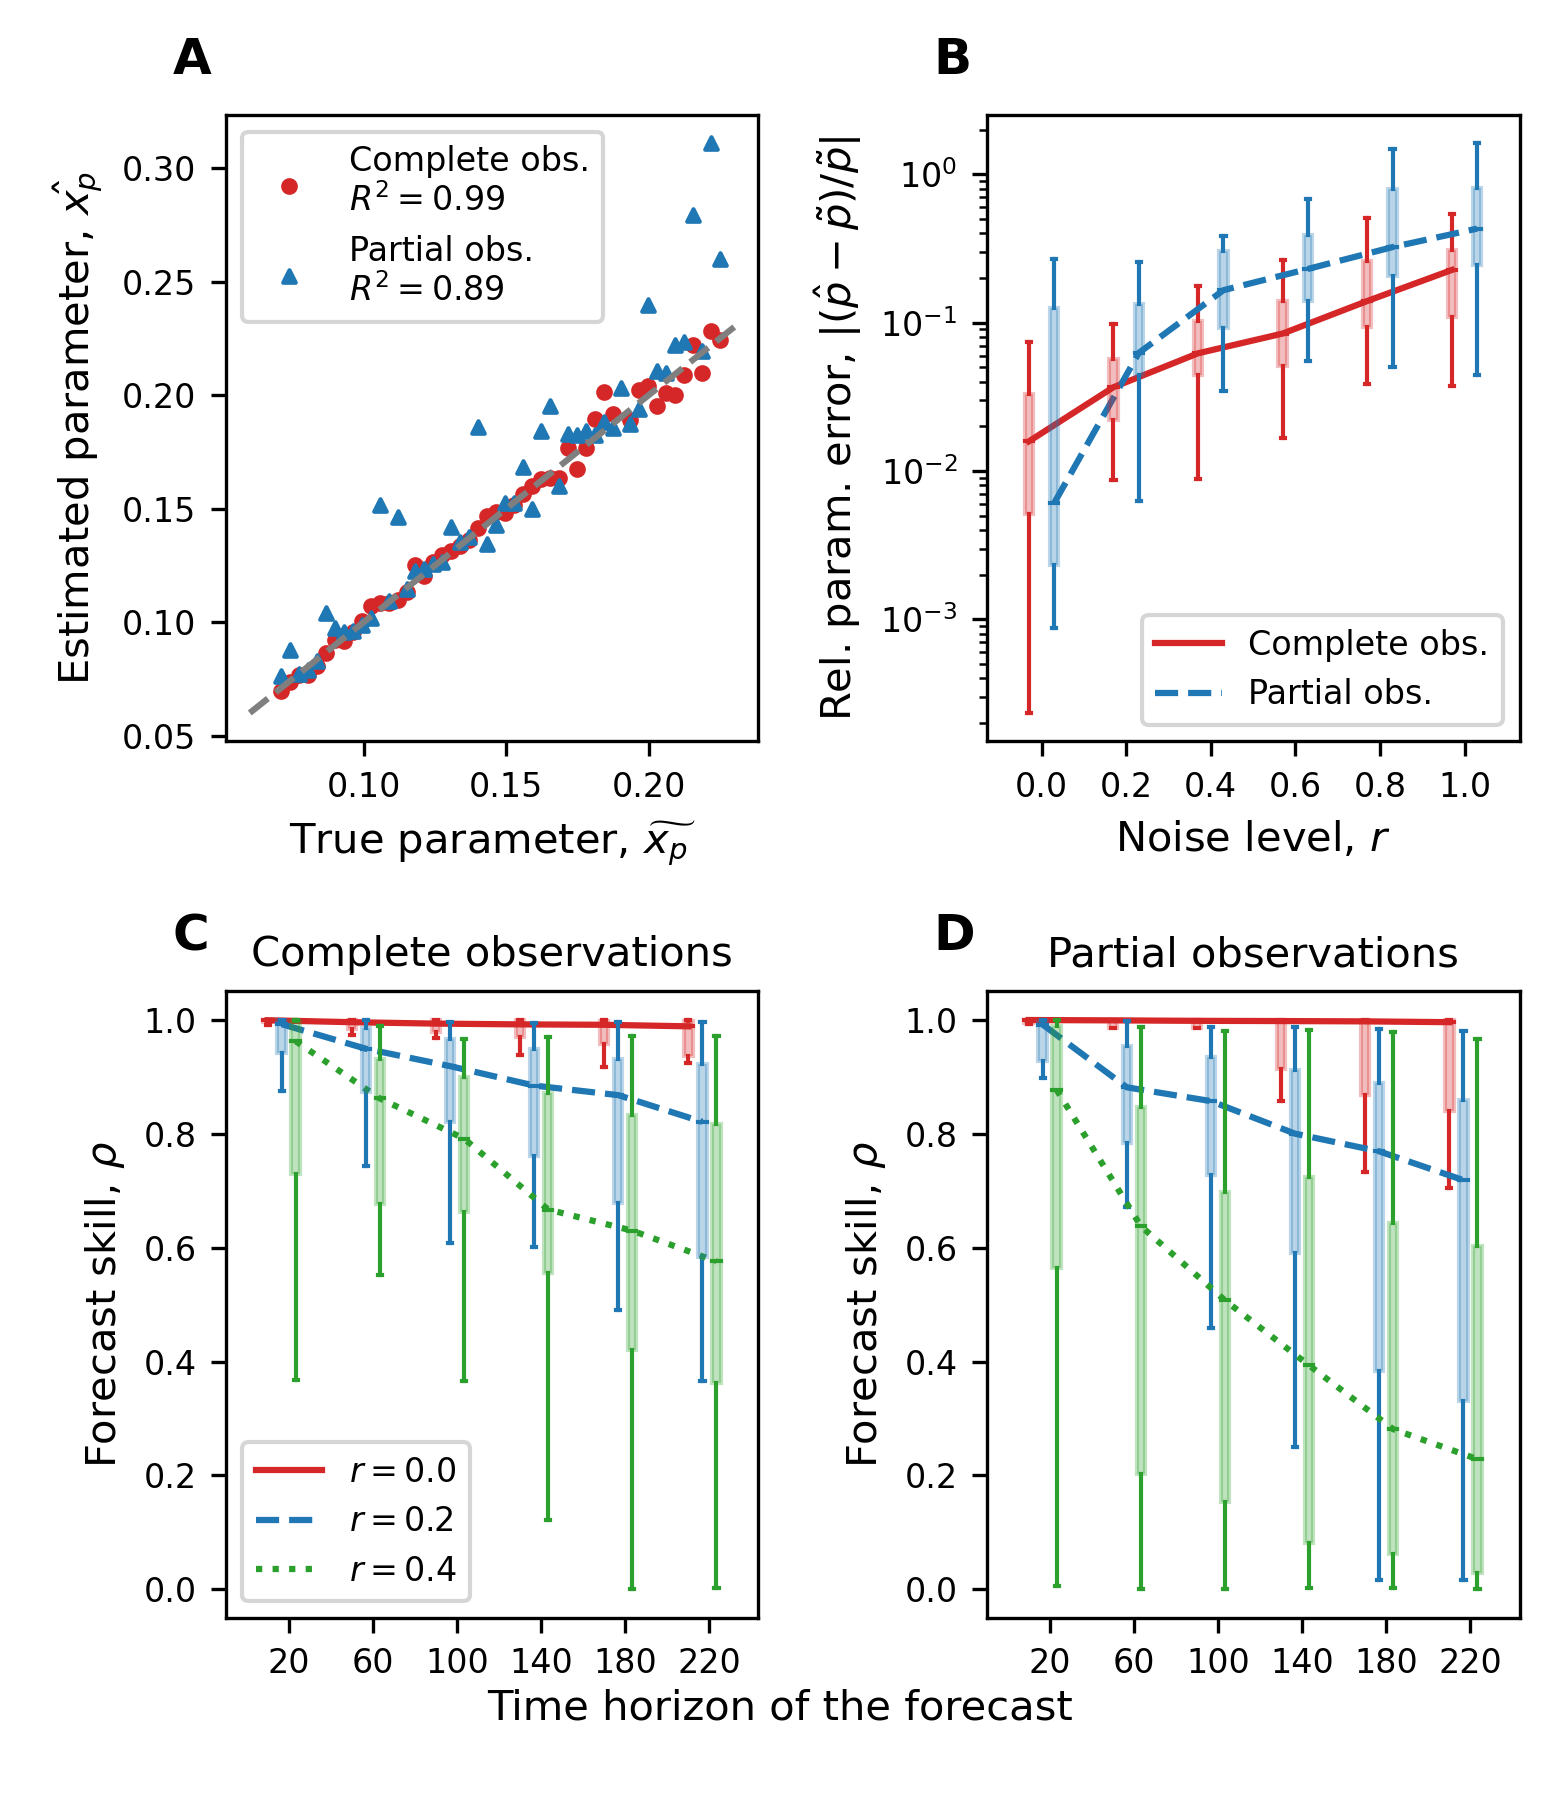
\includegraphics[]{figures/figure3.png}
    \caption{\textbf{Performance of the proposed ML framework for varying noise levels, under the complete and the partial observation setting.} 
    %
    \textbf{A} True parameter $\Tilde{x_P}$ against estimated parameter $\hat{x_P}$ for $r = 0.2$ under the complete and the partial observation setting. Although the parameter estimation is more accurate when complete observations of abundance are available, parameters show a fair fit when estimated with partial observations. 
    % 
    \textbf{B} Relative parameter error $\perr$ for varying noise levels under the setting of complete or partial observations. \textbf{B} supports the above observation for varying noise levels.
    %
    \textbf{C} Forecast skill $\rho^2$ of the trained model under the complete observation setting.
    %
    \textbf{D} Analogous data under the partial observation setting.
    %
    In \textbf{A}--\textbf{D}, the batch size is set to $m = 6$.}
    \label{fig:perfect_setting_noise}
\end{figure}
\FloatBarrier

\subsubsection{Capability of the ML framework to harness multiple time series}
We further investigate the ability of the ML framework to process and combine information from independent datasets. 
%
We reduce the time horizon of the observation data by setting the time series length to $K = 12$, generate two datasets comprising $S = 1$ and $S=6$ independent time series, respectively, -- obtained from independent ICs -- and set the number of batches for each time series $s$ to $M^{(s)} = 2$. In both the complete and partial observation settings, we find that the relative parameter error $\perr$ is consistently lower in the simulations with a larger number of time series (\cref{fig:perfect_setting_multiple_TS}\textbf{A}). The forecast skill is also consistently improved as more independent time series are processed (\cref{fig:perfect_setting_multiple_TS}\textbf{B}), and the forecast skill for long-term predictions considerably increases.
These results confirm the robustness of the ML framework against noise and partial observations, and show that the ML framework can efficiently harness the information from disparate observation datasets.
%

\begin{figure}[h]
    \centering
    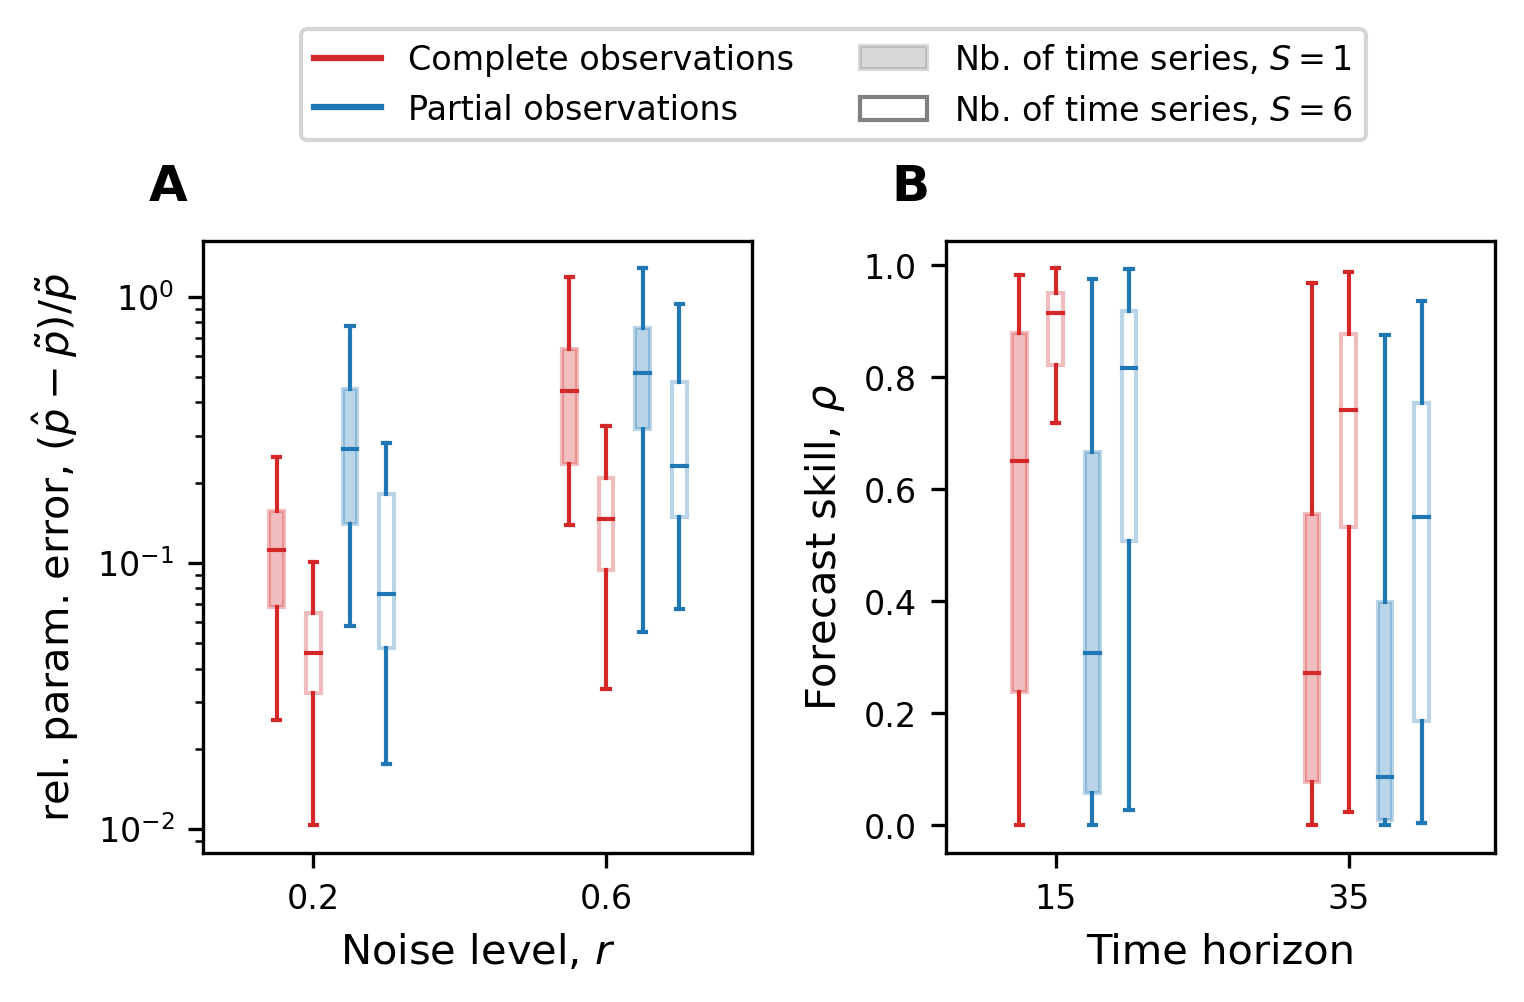
\includegraphics[]{figures/figure4.png}
    \caption{\textbf{Performance of the ML framework in processing and combining the information of multiple independent data sets.}
    %
    \textbf{A} Relative parameter error $\perr$ for different numbers of time series and levels of noise, under the complete and the partial observation setting. 
    %
    \textbf{B} Forecast skill for different numbers of time series and time horizons of the forecasts, under the complete and the partial observation setting. $r = 0.1$.
    %
    In \textbf{A}--\textbf{B}, $\perr$ decreases while $\rho^2$ increases as the number of time series processed increases, demonstrating the capacity of the ML framework to process and combine the information from independent time series.
    %
    In \textbf{A}--\textbf{B}, each box plot corresponds to 100 independent simulations where $\Tilde{x_P}$ varies $\Tilde{x_P} \in [0.071, 0.225]$, and the batch size is set to $m = 6$.
    }
    \label{fig:perfect_setting_multiple_TS}
\end{figure}
\FloatBarrier

\subsection{Elucidating mechanistic pathways}
\label{sec:model_comparision}
Finally, we relax the perfect-model assumption and investigate whether the ML framework can provide statistical support for the true generating model among several candidates with information-based model selection.
%
Specifically, we investigate whether the ML framework can detect omnivory from single observations of time series.
%
We generate multiple observation datasets from the omnivory variant model $\M_2$ for different omnivory strengths $\omega$ and noise levels $r$. We consider both the standard model $\M_1$ and the omnivory variant model $\M_2$ as two plausible candidate models (see \cref{fig:3species_foodchain_simple} for a graphical illustration of the models).
% 
We use the Akaike information criterion (AIC) to select the model with the strongest support in relation to the data \citep{Mangan2017}.
% 
In the specific case of our framework, we calculate the AIC as
\begin{equation}
    \AIC_{\M_i} = -2 \ln(p(\hat \theta, M_i | \by_{1:K})) + 2 k_{\M_i}
\end{equation}
% 
where $p(\hat \theta , \M_i| y_{1:K})$ corresponds to the maximum value of the likelihood of the model $\M_i$ given the data, and $k_{\M_i}$ is the number of parameters in the model $\M_i$.
% 
The AIC ranks the most probable models by penalizing complexity to balance information loss and parsimony, where candidate models with the lowest scores are ranked as the most likely.
%
We consider the Akaike weights $w_{\M_i} = \tfrac{\exp(- \Delta \AIC_{\M_i}/2)}{\sum_j \exp(- \Delta \AIC_{\M_j} / 2)}$, where $\Delta \AIC_{\M_i} = \AIC_{\M_i} - \min_{j} \AIC_{\M_j}$, which can be directly interpreted as the probability that $\M_i$ is the most appropriate model given the data (see \citep{Burnham2002}).
%
We expect that the Akaike weights provide support for the generating model $\M_2$ only across values where $\omega > 0$, as $\M_1$ is equivalent to $\M_2$ when $\omega = 0$ and $\M_2$ is penalized by its three additional parameters.

%%
In the complete observation setting, for moderate observational noise ($r = 0.1$) we find that $\M_1$ is given strong support for $\omega < 0.07$ ($w_{\M_1} > 98\%$) and that $\M_2$ if favored for $\omega > 0.08$ ($w_{\M_2} > 99\%$), providing overall strong support for the true model over a large range of $\omega$ values (\cref{fig:AIC_likelihood_comparision_3-compartments-model}\textbf{A}). 
%
As the observational noise increases the support strength naturally decreases, leading to an increased range of $\omega$ values where the simplest model $\M_1$ is favored or where no model is given strong support (\cref{fig:AIC_likelihood_comparision_3-compartments-model}\textbf{B}-\textbf{C}).
% 
On the other hand, in the partial observation setting, the lack of data prevents the correct estimation of the omnivory variant model parameters, leading model $\M_1$ to be supported for an even larger range of $\omega$ values (\cref{model_selection_1sp}).

%%
Overall, the ML framework provides statistical support for the model embedding the most appropriate hypotheses given the available data. With appropriate data, the proposed ML framework can therefore elucidate mechanistic pathways and infer ecological processes by utilizing information-based model selection.

\begin{figure}[h]
    \centering
    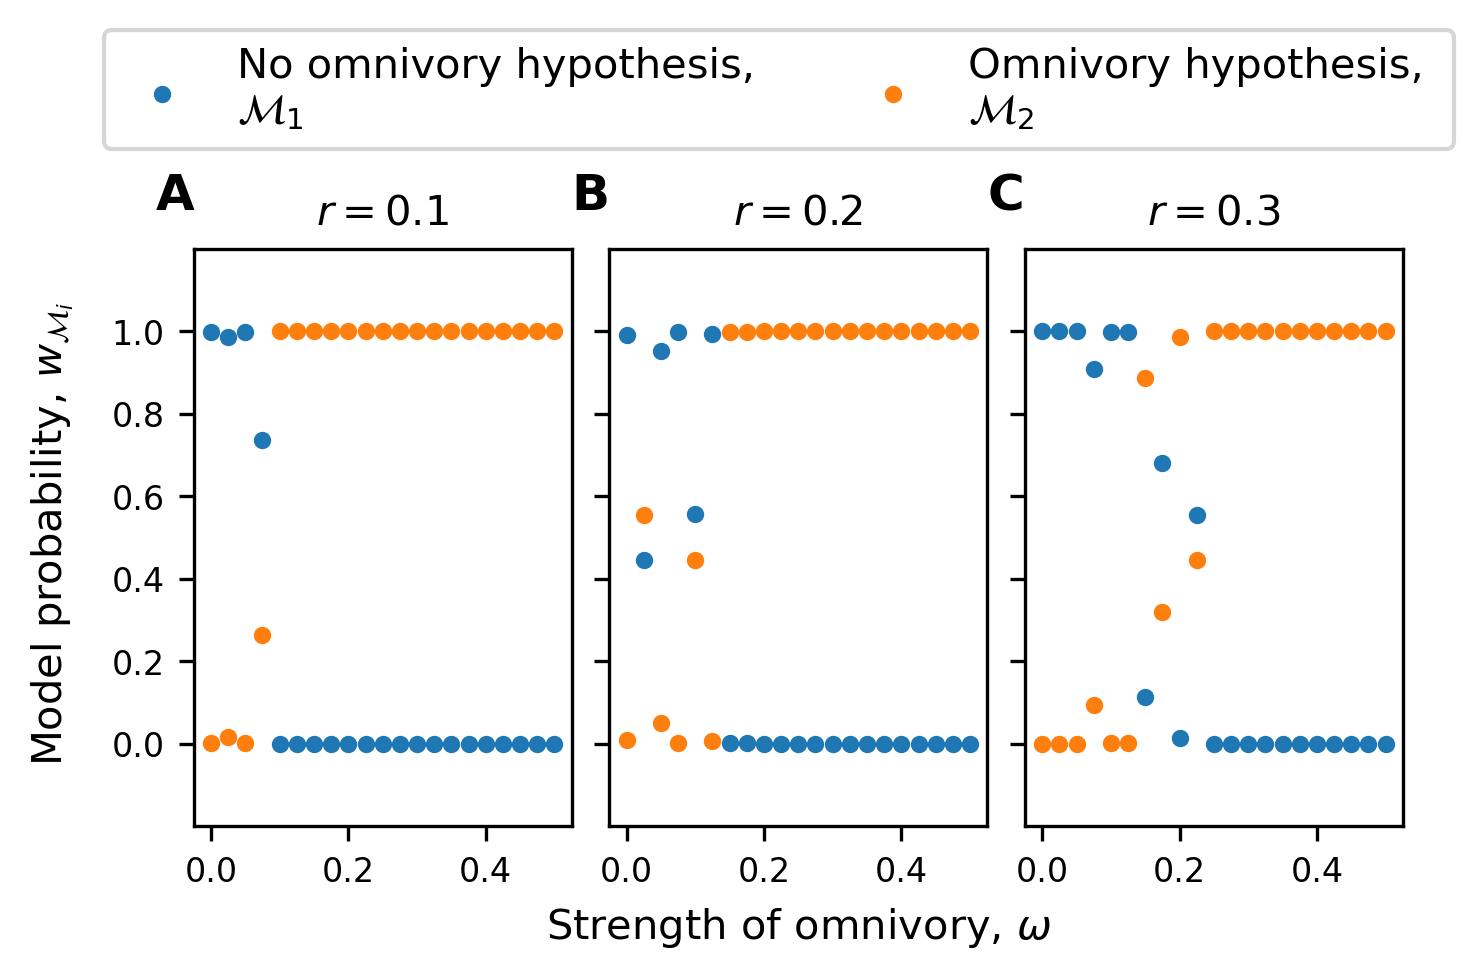
\includegraphics[]{figures/figure5.png}
    \caption{\textbf{Performance of the ML framework in supporting the predator omnivory hypothesis in a food web.}
    %
   \textbf{A}--\textbf{C} Hypothesis testing for levels of noise $r=0.1, 0.2, 0.3$. Blue dots correspond to $w_{\M_1}$, the Akaike weights of the simple food-web model, and orange dots correspond to $w_{\M_2} = 1 - w_{\M_1}$, the Aikaike weights of the omnivory model, which can be interpreted as model probabilities. 
    %   
   \textbf{A}--\textbf{C} indicate that the ML framework can detect omnivory, as the omnivory model $\M_2$ is given strong support ($w_{\M_2} > 99\%$) for most of the $\omega$ range investigated.
    }
    \label{fig:AIC_likelihood_comparision_3-compartments-model}
\end{figure}

\FloatBarrier

\section{Discussion}\label{sec:discussion}

%% summary and comparison with other methods
We propose a ML framework combining a mini-batch method inspired by multiple shooting methods \citep{Pisarenko2004} with automatic differentiation \citep{Rackauckas2020a} and state-of-the-art variational optimizers \citep{Kingma2014} to efficiently and accurately parametrize complex dynamical models. 
% 
We show formally that splitting the data into mini-batches with a short time horizon regularizes the loss function associated with dynamical models characterized by complex dynamics, such as chaotic dynamics and limit cycles (\cref{secSI:supmat}). We demonstrate numerically that this reformulation ensures the success of gradient-based optimizers to parametrize ecosystem models (\cref{fig:training_on_mini-batches,fig:perfect_setting_noise,fig:perfect_setting_multiple_TS}).
% 
This mini-batch method is also relevant beyond variational methods and applies to any inferential method navigating the posterior landscape, such as evolutionary algorithms \citep{wilke2001evolution,Rodriguez-Fernandez2006} or Markov Chain Monte Carlo methods \citep{Lignell2013,Higgins2010,Xu2006,Fiechter2013,Rosenbaum2019}.
% 
The proposed approach is particularly relevant for the parametrization of ecosystem models incorporating realistic ecological and adaptive mechanisms \citep{Urban2016}, which are generally associated with strong nonlinearities due to the complexity of processes linking interacting ecological compartments \citep{Bjornstad2001,Hastings1993,Huisman1999,Beninca2008}. It further integrates the practical constraints of available ecological datasets \citep{Dornelas2018}, accommodating incomplete, noisy, shallow and independent observation data.
%%
Overall, the ML framework successfully blends ML methods with mechanistic ecosystem models to learn from ecological time series, and it could therefore improve our quantitative understanding of ecosystem dynamics and help to anticipate their responses to global changes \citep{Urban2016}.

%%
Our work contributes to the ongoing effort to better assimilate observational data into mechanistic models \citep{Schartau2017,Raissi2019,Kashinath2021}, with a specific focus on the parametrization of ecosystem models with strong nonlinearities.
%
Recently, \citep{Yazdani2020} proposed an alternative framework dubbed "systems biology informed deep learning", where a neural network is fitted to the data and the additional mechanistic model constraints are integrated. This alternative framework extends previous colocation methods \citep{Ramsay2007,Cao2008} and has the advantage of being able to parametrize stochastic models. As it requires the selection of a neural network architecture and a "goodness of fit" parameter, it nevertheless imposes an additional layer of complexity, which might negatively affect the model parametrization  \citep{Yazdani2020}. 
% 
In contrast, the ML framework proposed here trains the model directly against data, using automatic differentiation and sensitivity analysis in order to apply variational optimizers directly to the model simulations. This makes it possible to bypass the use of neural networks, rendering the parametrization process simpler and more amenable to model selection \citep{Ramsay2007}. 
% 

%%
By integrating the practical constraints imposed by ecological datasets, the ML framework can learn from short time series with partial and noisy observations (\cref{fig:perfect_setting_noise,fig:perfect_setting_multiple_TS}). 
% 
Local ecosystem surveys, such as marine trawling surveys or local terrestrial surveys (\citep{Pinsky2013,Dornelas2018,Burrows2019} and references therein), provide time series that are generally shallow in time but composed of many replicates \citep{Hsieh2008,Clark2015}, in part due to the practical difficulties of long-term monitoring \citep{Ye2016}. 
% 
Our results show that the inclusion of multiple independent time series in the training dataset reduces the error in the parameter estimates and increases the forecast skill (\cref{fig:perfect_setting_multiple_TS}). This indicates that the proposed ML framework could, in practice, efficiently harness the information available in current ecological datasets.
% 
Instead of directly comparing simulated and observed data, matching time-averaged statistics between observations and simulations (e.g. means and covariances) could further yield an improved assimilation of observations from diverse data sources, such as global observations of productivity from satellites and local surveys, as proposed for climate models \citep{Schneider2017}.
% 
Overall, the proposed ML framework accommodates the specificities of current ecological time series and can improve the assimilation of ecological data into mechanistic ecosystem models.

%%
Our work can help elucidate mechanistic pathways by contrasting hypotheses embedded in model variants.
%
Using information-criterion-based model selection, we demonstrate with a case study that the ML framework is able to provide statistical support for the true generating model among two different candidates (\cref{fig:AIC_likelihood_comparision_3-compartments-model}).
% 
Importantly, the ML framework can perform model selection on complex models, incorporating key mechanisms such as trait--species interactions, evolutionary potential and responses to environmental conditions, which have been shown to be important in mediating ecosystem dynamics and must be refined in models to improve predictive accuracy \citep{Urban2016}.
% 
The ML framework can therefore lead to the improvement of current ecosystem models and knowledge, which is crucially needed given that key ecological processes are only partially described in most ecosystem models \citep{Schartau2017}.
% 
AIC can also be used to ensure the interpretability of the model parameters, and should be preferred to estimating the parameter uncertainty through e.g. the Cramer Rao inqequality \citep{Burnham2002}: by favouring models with less complexity, model selection techniques disqualify uninformative parameters to ensure interpretability \citep{Burnham2002}. This has the extra benefit of reducing the dimensionality of the parameter space, hence improving the estimation of other parameters. 
%
Following recent novel approaches to investigate ecological hypotheses \citep{Curtsdotter2019}, our method contributes to the development of a process understanding of ecosystem functions and provides a path forward to better link ecological theory and data.

%%
The proposed approach still presents a set of limitations, which might hamper its success under specific situations. 
% 
First, while the use of mini-batches smooths the loss surface and ensures better convergence, it also flattens the loss surface around the true parameter value, which consequently deteriorates the precision of the inferred parameters because the loss function takes similar values in an extended neighbourhood of the true parameters. 
% More formally, the curvature of the loss function around the true parameters is decreased, which deteriorates the fisher information of the time series (see \cref{secSI:supmat}). 
To circumvent this issue, iterative training can be performed, where the learning is initiated by a short batch length $K^{(s)}$ to identify the region with the most probable parameters, and in subsequent iterations the batch length is increased to improve the precision of the inference. 
% 
Iterative training could also improve the lack of statistical support obtained in hypothesis testing experiments (see simulations in \cref{fig:AIC_likelihood_comparision_3-compartments-model,model_selection_1sp} where none of the models is given statistical support), as it would increase differences in likelihood for parameter values around the neighbourhood of the true parameter values.
% 
Second, our results highlight that the data might not provide enough constraints for a correct parametrization (\cref{fig:perfect_setting_multiple_TS}, partial observation setting and $S=1$). Pre-experimental analyses with simulated synthetic data might therefore be required to design the sampling protocol and campaign to ensure an adequate sampling effort \citep{Banks2017,Laubmeier2018}. % This can be done with Fisher information.
%
Third, while in \cref{eq:ML-framework} it is assumed that the parameter values are the same across the time series, strong regional variability might also be observed among the spatially replicated data, causing parameter values to vary across the replicates. The knowledge of this variability could motivate partial pooling \citep{Beaumont2010} or parametrization of the parameters in terms of environmental conditions \citep{Pahlow2008}, to account for the independence of the parameter values across the replicates.
%
Finally, while the proposed ML framework greatly improves convergence, it could still be that -- even with a large amount of data -- poor initial parameter estimates, a large number of free parameters, or high noise levels prevent convergence to the true minimum. Performing multiple runs with varying initial parameter estimates can ensure that the maximum a priori estimate is reliable. If this is not the case, stochasticity could further be introduced within the ML framework to prevent the convergence to local minima, where only a subset of mini-batches are fitted at each epoch \citep{bottou2012stochastic}.

\section{Conclusion}
We proposed a ML framework based on a mini-batch method combined with automatic differentiation and state-of-the-art optimizers to estimate the parameters and improve the forecast skill of complex ecosystem models from observation data.
% 
The ML framework was benchmarked with a realistic ecosystem model characterized by strong nonlinearities and delivered excellent performance, accommodating the practical constraints imposed by the quality and availability of ecological datasets.  Our experiments have further illustrated the ability of the ML framework to discriminate between several candidate models, enabling the testing of ecological theories against data and the improvement of current mechanistic models.
% 
Given the increasing number of ecological datasets following the development of monitoring technologies such as environmental DNA \citep{Ruppert2019}, remote sensing \citep{Jetz2019}, bioaccoustics \citep{Aide2013}, and citizen observations \citep{GBIF}, the proposed ML framework opens up new opportunities for the quantitative investigation of current ecosystem functions \citep{Curtsdotter2019} and the prediction of ecosystem responses to increasing disruptions \citep{Urban2016}.

\section{Acknowledgements}
% The authors thank Thomas Poulet and François Duchene for helpful discussions and comments.
L.P. and V.B. were supported by the SNF grant 310030E\_205556. P.V.A. was supported by an ETH postdoctoral fellowship. 

\section{Code availability}
The ML framework is implemented in the multi-purpose Julia package \textbf{MiniBatchInference.jl} available at \href{https://github.com/vboussange/MiniBatchInference.jl}{https://github.com/vboussange/MiniBatchInference.jl}, and the simulation code is available at \href{https://github.com/vboussange/mini-batching-ecological-data}{https://github.com/\linebreak vboussange/mini-batching-ecological-data}.

% \printbibliography[heading=subbibliography]